\chapter{About the data and research design}\label{ch:3}

%section 3.1 begins %%%%%%%%%%%%%%%%%%%%%%%%%%%%%%%%%%%%%%%%%%%%%%%%%%%%%%%%%%%%%%%%%%%%
\section{Introduction}
This research had two chief aims. The first aim was to develop a novel tripartite methodological analysis tool, with which the second aim could be addressed. The second aim involved an attempt to bring an end to the contention surrounding the origin of the \ili{English} lexico-phonetic element in \ili{Sranan}; i.e. whether this origin was best explained by a \isi{pan-dialectal account} of origin, or a \isi{mono-dialectal account} of origin. In attempting to accomplish the above-mentioned aims, the research relied heavily on three types of secondary data. These were \ili{Sranan} data, \ili{English} \isi{dialect geography} data and \isi{historical data} surrounding 17\textsuperscript{th} century migration from \isi{England} to the \isi{Caribbean} and South America.
%section 3.1 ends %%%%%%%%%%%%%%%%%%%%%%%%%%%%%%%%%%%%%%%%%%%%%%%%%%%%%%%%%%%%%%%%%%%%

%section 3.2 starts %%%%%%%%%%%%%%%%%%%%%%%%%%%%%%%%%%%%%%%%%%%%%%%%%%%%%%%%%%%%%%%%%%%%
\section{Data sources}\label{3.2}
\subsection{Sranan data} \label{3.2.1}
The main source of data on \ili{Sranan} that was used to conduct this research was the \emph{Dictionary of \ili{Sranan} Tongo} \citep{Wilner07, Wilner03, Wilner92}. This was supplemented by four complementary sources in the form of the wordlists of Stichting Volkslectuur \citep{Stichting80},  \citet{Schumann83}, \citet{Fermin69}, and \citet{Herlein18}. Because of the varying periods in which the four wordlists and dictionary were compiled, the spelling conventions used across them varied considerably. The phone [u], for example, was represented as $\langle$oe$\rangle$ in Stichting Volkslectuur  \citep{Stichting80} but as $\langle$u$\rangle$ in  \citet{Wilner03}. The $\langle$oe$\rangle$ form used in Stichting Volkslectuur  \citep{Stichting80} is possibly \ili{Dutch}-based, whereas the $\langle$u$\rangle$ used in  \citet{Wilner03} is possibly based on the International Phonetic Alphabet (IPA).

Two steps were taken to deal with this issue of variability across the \ili{Sranan} data sources. First, Smith's  \isi{historical phonology} work, \emph{The Genesis of the \ili{Creole} Languages of Surinam} \citep{Smith87}, was used to help reconstruct the actual phones that each writing convention was representing. \citet{Smith87} provided a very systematic and detailed discussion of how to interpret the phonetic information behind the graphemes in each of the wordlists. For the purpose of uniformity, the phonetic forms that these graphemes represented were then transcribed in accordance with the conventions of the revised 2005 IPA. Second, where there was a variation in the lexico-phonetic shape of a word found across these sources, preference was given to the oldest variant; the oldest variant was selected because the aim was to work with items that would represent, as much as possible, what \ili{Sranan} might have looked like in the 17\textsuperscript{th} century. This was an important step since the intention was to compare not just the lexical form but also phonetic composition of \ili{Sranan} words and their potential \ili{English} etyma. Accordingly, the \ili{English} dialectal data, discussed in \sectref{3.2.2}, were also transcribed using the above-mentioned revised IPA convention.

\subsection{English dialect data} \label{3.2.2}
\begin{quote}
Rarely are the characteristics of a language uniform across the region where it is used. Internal spatial variations in a linguistic region are called \isi{dialects}, and language geographers study these variations in an effort to distinguish and understand the geographic qualities of dialect use ... \citep[209]{Hanks11}.
\end{quote}

Dialect geographies shed light on lexical, phonological, syntactic and morphological diversity of individual \isi{languages} over geographic spaces. These works allow linguists to generate linguistic atlases, i.e. maps that sectionalise a particular geographic space according to dialectal differences and similarities, as opposed to geographic and/or political boundaries. The importance of \ili{English} \isi{dialect geography} to this work was twofold. First, it provided lexical and phonetic dialectal data for the \ili{English} etyma relevant to the \ili{Sranan} reflexes of \ili{English} origin. Second, it allowed for the identification of the potential regional dialectal variants and sources for these items.

There are four main dialect geographies for the \ili{English} \isi{dialects} spoken in the \ili{British} Isles. These are: the \emph{Survey of Anglo-\ili{Welsh} Dialects} \citep{Parry77, Parry79} and \citet{Penhallurick91}, the \emph{Linguistic Survey of Scotland} \citep{Mather75}, \emph{A Sound Atlas of \ili{Irish} English} \citep{Hickey04} and the \emph{Survey of \ili{English} Dialects} \citep{Orton6271}.

The Survey of Anglo-\ili{Welsh} \isi{Dialects} ``... is the most comprehensive collection of \ili{Welsh} \ili{English} data ... [archived] at the Department of \ili{English}, University of Wales, Swansea...'' This collection of \ili{Welsh} data is attributed to two researchers. The first is David Parry, under whose supervision ``... material was collected in rural areas of Wales between 1968 and 1982 ... and in urban areas between 1985 and 1987 \citep[100]{Penhallurick04}. The second researcher is Robert Penhallurick who, in 1991, carried out a survey in the north of Wales, specifically to collect data on the conservative rural \ili{English} dialect spoken in the counties of Gwynedd and Clwyd \citep{Penhallurick91}.

The Linguistic Survey of Scotland, which was undertaken by  \citet{Mather75}, does not necessarily qualify as \isi{dialect geography}. The data contained in this work was the result of a postal questionnaire survey that, according to  \citet[225]{Macaulay77}, suffered from a ``... loss of phonological information...'' and also from fundamental design flaws in how the sample population was selected. Head teachers from across Scotland, as opposed to trained researchers, were instructed to hand out some of the questionnaires to ``... middle-aged or older ... life-long inhabitants...'' in their districts \citep[14]{Macaulay77}.

\citet{Henry58} in his ``Preliminary Report'' outlined proposals to develop a \isi{dialect geography} of \ili{Irish} \ili{English}. His preliminary objectives were not achieved and the result was only a minute collection of word charts from within the agricultural sphere \citep{Corrigan10}. There is however, contemporary work that was produced by \citet{Hickey04}, which was built on over 1,500 anonymous vernacular samples, audio recorded from 1,200 informants across rural and metropolitan settings in all thirty-two counties in Ireland \citep{Corrigan10, Hickey04}. Hickey's \emph{A Sound Atlas of \ili{Irish} English} was created to provide a present-day depiction of \ili{Irish} \ili{English}, specifically as it related to the language use of the younger generation of \ili{Irish} \ili{English} speakers \citep{Hickey04}.

The final \isi{dialect geography}, the \emph{Survey of \ili{English} Dialects}, hereafter \textsc{sed}, was undertaken by \citet{Orton6271} between 1962 and 1971, via audio recorded sessions done by trained researchers, using an orally administered questionnaire. The questionnaire consisted of  ``... 1,322 questions of which 387 are for phonological, 128 for morphological, and 77 for syntactical purposes [respectively], the remaining 730 being mainly concerned with the \isi{lexicon}'' \citep[15]{Orton62}.

History tells us that immigrants to the 17\textsuperscript{th} century \ili{English} colonies came from Ireland, Scotland, Wales and \isi{England}. However, the aim was to pinpoint \ili{Sranan}'s earliest \ili{English} input and for this reason the study focused only on identifying \ili{Sranan}'s early \ili{English} \isi{dialectal origin}(s) from within \isi{England}. There are a number of reasons for having only dealt with 17\textsuperscript{th} century \isi{England}. As noted earlier, some of these included the fact that major \ili{Irish} and \ili{Scottish} migration to the American colonies did not occur until the late 18\textsuperscript{th} century, i.e. 1718--1785 for the \ili{Irish} \citep{Griffin01} and 1716 for the Scots (see \citealt{Dobson05}), respectively. By these periods \isi{Suriname} was no longer an \ili{English} held colony, having already been ceded to the \ili{Dutch} in 1667. Also, there were issues of comparability between the dialect geographies. \emph{The Sound Atlas of \ili{Irish} English}, for example, only provided present day \ili{Irish} \ili{English} data as opposed to more archaic versions of this language \citep{Hickey04}; the \ili{Scottish} \ili{English} \isi{dialect geography} could not be classified as a \isi{dialect geography} proper and it did not provide phonological data from which cross-dialectal comparisons could be made. Also, according to  \citet{Macaulay77}, it suffered from fundamental design flaws in the selection of the sample population; untrained data collectors, i.e. head teachers from across Scotland were instructed to hand out some of the questionnaires to ``... middle-aged or older ... life-long inhabitants...'' in their districts \citep[14]{Macaulay77}, there was no means by which to determine whether the teachers themselves did not fill out some of the questionnaires. In addition, the historical literature indicated that of the migrants to the American colonies during the period in which \isi{Suriname} was a \ili{British} colony, i.e. 1650--1667, the vast majority came from within the southwestern \isi{England} counties of Somerset, Gloucestershire, Wiltshire and Monmouthshire \citep{Burg95, Schaefer98}, the latter being a \ili{Welsh} county bordering Herefordshire and Gloucestershire to the west, which was also surveyed in the \textsc{sed} (see \sectref{3.2.2.1}).

The fact that \ili{Irish} \ili{English}, \ili{Scottish} \ili{English} and \ili{Welsh} \ili{English} \isi{dialects} formed a part of the input in \ili{English}-based \isi{Creoles} of the Americas \citep{Mufwene01, Smith87} cannot be downplayed. However, for the above-mentioned reasons The \emph{Survey of \ili{English} Dialects} was the main \isi{dialect geography} source used in this research.

\subsubsection{The survey of English dialects} \label{3.2.2.1}
\citet{Orton62} held traditional regional \ili{English} \isi{dialects} as being best preserved by farming communities, and as such ``... the questionnaire [used in the \textsc{sed}, was] constructed for the farmer''  \citep[44]{Orton62}. Since this was the case, the questions asked dealt mainly with ``... husbandry, home life and nature... [and areas such as] ... fishing, mining, weaving... [were] ... excluded as being too technical and not universal'' \citep[44]{Orton62}. Orton believed that responses to questions of the above-mentioned types ``... would [have] shed light on the lexical, phonological and morphological diversity of spoken \ili{English}'' (\citeauthor{lavc09}).

The \textsc{sed} was conducted in 313 localities across \isi{England} and parts of Wales. This also included two localities in the Isle of Man. The localities in Wales were surveyed because they border localities in the west of \isi{England} \citep{Orton6271} and \isi{dialects} of \ili{Welsh} \ili{English} in this region were influenced by south-west \isi{England} \ili{English} speakers, who migrated across the Bristol Channel from Somersetshire and Devon, from as early as the 12\textsuperscript{th} century \citep{Penhallurick04}. Also, what we call Wales and \isi{England} are political terms \citep{Nicholas72}, as opposed to linguistic ones. Consequently, political lines indicated on a map do not correspond to actual physical boundaries, such as mountains, which separate people who live in localities that border each other. In other words, what is spoken in a given region is not determined by how that region is politically divided \citep{Orton6271}.

According to \citet{Orton62}, the localities were selected according to their ``... geographical isolativity and relativity to each other... [with] ... preference given to agricultural communities that had a fairly stable population of about 500 inhabitants for a century or so'' \citep[15]{Orton62}. The survey was geared towards eliciting archaic, ``lexical features... in the form of ... phonological variants... and grammatical features'' \citep[45]{Orton62}. Since this was their goal, the researchers took as their target population ``... men and wom\-en, sixty and over...'' \citep[45]{Orton62} because they were considered to be more likely to best preserve the traditional dialect.

The \textsc{sed} was to be published in five parts under the headings (A): Introduction, (B): Basic Material, (C): Selected Incidental Material, (D): Linguistic Atlas of \isi{England} and (E): Phonetic Transcriptions, of the audio recorded interviews \citep{Orton62}. However, to date, only parts (A), (B) and (D) can be found in print, because after the publication of the basic material and possibly due to the death of Orton in 1975, neither Parts (C) nor (E) were published.

Part (D) was itself not published as a single atlas at first, ``but in the form of six, often parallel and overlapping atlases ... the earliest of these [being] Kolb's \citep{Kolb79}'  \emph{Atlas of \ili{English} Sounds}'' \citep[12]{Fischer91}. Orton's originally envisioned Linguistic Atlas of \isi{England} was not published until 1978 and in keeping with his (Orton's) original wish, it contained ``... phonological, lexical, morphological and syntactic maps...'' based on the responses of the interviewees that could be found in the Basic Material \citep[12]{Fischer91}.

This current research relied heavily on Parts (A): Introduction, (B): Basic Material and (D): Linguistic Atlas of \isi{England}. Part (A): Introduction contained an index, referred to as the `List of Key-words', which highlighted the particular feature/variable that \citet{Orton62} were attempting to capture from the questions asked during the survey. This index indicated whether a particular feature/variable was asked for, where it was asked for and why. As it relates to the `why', the Index used three symbols, an asterisk \textasteriskcentered, an obelisk \textdagger, and a double obelisk \textdaggerdbl. According to \citet{Orton62}, an asterisk indicated ``... phonological, an obelisk morphological, and a double obelisk syntactical significance'' \cite[47]{Orton62}. ``Key-word'' items that bore none of the above-mentioned marks meant that they were of lexical significance only. Part (B): Basic Material consists of four volumes in three parts each. These four volumes -- the \emph{Six Northern Localities and Man}, the \emph{West Midland Counties}, the \emph{East Midland \isi{Counties} and East Anglia} and the \emph{Southern Counties} -- contained the variant responses to the questions asked during the survey. All responses were given in the then contemporary, 1951 version of the IPA. These books therefore provided access to the several lexical and phonetic variants of a given item in the index of ``Key-words''. Part (D): The Linguistic Atlas presented a visual representation of the geographic distributions of the ``Key-word'' items and their lexical and phonetic variants (see \sectref{3.3.1}).

\subsection{The historical data} \label{3.2.3}
The principal source of \ili{English} migrants to the \ili{British} colonies, before 1776, consisted of indentured servants \citep{Esposito82}. This large body of migrants included:

\begin{enumerate}
\item{political prisoners, i.e. deported Royalists of the King's army. Between 1645 and 1650 the \ili{English} Civil War contributed at least 8,000 indentured servants to the West Indian colonies. This increase in the numbers of servants ran concurrent with the sugar boom that was being experienced in the 1640s and 1650s \citep{Brewer96};}
\item{despairing \ili{English} countrymen searching for a better life far from a socially and economically unstable \isi{England}.}
\end{enumerate}

Determining the origin of these indentured servants involved scrutiny of a number of historical documents. The main body of \isi{historical data} was taken from \emph{The Complete Book of Emigrants: 1607--1660} \citep{Coldham92, Coldham87}, \emph{The Bristol Registers of Servants Sent to Foreign Plantations, 1654--1686} \citep{Coldham88}, and the \emph{Virtual Jamestown, Virginia Center for Digital History} (\citeauthor{vcdh}) and the \emph{\ili{British} History Online} databases (\citeauthor{bho09}), respectively. The second of the latter two sources afforded me access to documents such as the \emph{Calendar of State Papers \isi{Colonial}, America and the West Indies}. The \emph{Calendar of State Papers}, which can be found in the \ili{British} National Archives, is a set of some 1,000 historical papers concerning 16\textsuperscript{th} to 18\textsuperscript{th} century \ili{English} activities in the American, Canadian, and West Indian colonies.

\emph{The Complete Book of Emigrants: 1607--1660} ``... was conceived as an attempt to bring together from as many \ili{English} sources ... a comprehensive account of emigration to the New World from its beginnings to 1660 ...'' \citep[vii]{Coldham87}. The book's content was compiled solely from \ili{English} historical records and not \ili{Irish}, \ili{Welsh}, \ili{Scottish} or American sources \citep{Coldham92, Coldham87}. One of  Coldham's (\citeyear{Coldham92, Coldham87}) sources included the \emph{\isi{Colonial} State Papers}; other sources included the \emph{Port Books of London} (\textsc{lva}), which provided information concerning indentured servant migration from London, to its American colonies within the period 1607--1660 \citep{Coldham92, Coldham87}.

\emph{The Bristol Register of Servants sent to Foreign Plantations}, originally referred to as the \emph{`Tolzey Book of Indentures'}, contained the systematic records of the indentures of over 10,000 \ili{English} migrants. These were migrants who left from the port of Bristol, between 1654 and 1686, when the trade in indentured servants had reached its peak \citep{Smith47, Morgan93}. The original Tolzey Book or \emph{Council Book}, which was entitled \emph{Servants to Foreign Plantations}, consisted of two leather-bound volumes that can be found in the archives of the Corporation of the City of Bristol in \isi{England}. In 1988 Peter Wilson Coldham compiled the set of records found in this two-part volume document, and made them accessible via the book, \emph{The Bristol Registers of Servants Sent to Foreign Plantations, 1654--1686} \citep{Coldham88}.

In this book, i.e. \emph{The Bristol Registers of Servants Sent to Foreign Plantations, 1654--1686}, \citet{Coldham88}, as he did in \emph{The Complete Book of Emigrants: 1607--1660} \citep{Coldham92, Coldham87}, provided information about indentured servants' names, dates of departure, destinations and the localities across \isi{England} and the Isle of Man from which they were migrating between the years 1654 and 1686 \citep{Sacks93}. It is from this source that the  \emph{Virtual Jamestown, Virginia Center for Digital History} (\citeauthor{vcdh}), created the online electronic registers database, which alongside Coldham's (\citeyear{Coldham92, Coldham87}) original work, was heavily consulted in carrying out this research.

\emph{\ili{British} History Online} is an online ``digital library containing ... the core printed primary and secondary sources for the medieval and modern history of the \ili{British} Isles... [It was] ... created by the Institute of Historical Research and the History of Parliament Trust and is ran by the Institute of Historical Research -- the centre for the study of history in the United Kingdom -- at the University of London''  (\citeauthor{bho09}). This digital online library resource lived up to the aims of the Institute by having afforded me access to ``... highly accurate digital versions of the core works of \ili{British} history...'' (\citeauthor{bho09}) such as the 17\textsuperscript{th} century, \emph{Calendar of State Papers, \isi{Colonial} America and West Indies} documents. The data from these state papers, and the data collected from the above-discussed sources did their part in providing relevant answers to three questions that were asked of the historical sources. These questions were as follows:

\begin{enumerate}
\item{ Can we establish a chain of migration from \isi{England} to \isi{Suriname}, between the years 1650 and 1667? Within these years \isi{Suriname} was settled by the \ili{English} and subsequently lost to the \ili{Dutch}. After 1667 \ili{English} migration to \isi{Suriname} had ceased (see discussion in \chapref{ch:6}).}
\item{Can we establish a chain of migration from \isi{England}, within the same time span mentioned in (1.), to the \ili{English} colonies in the \isi{Caribbean} and subsequently \isi{Suriname}?}
\item{If the answer to (1.) and/or (2.) is in the affirmative, then what proportion of the total number of migrants to the \isi{Caribbean}, including \isi{Suriname}, is from the various localities across \isi{England}?}
\end{enumerate}


\subsection{Limitations}
This study, as is the case with any type of research, suffers from a number of shortcomings. One shortcoming is that because of the time of the \textsc{sed}, i.e. 1950 to 1961, there is a circa 300 year gap between when this survey was done and when the first emigrants to \isi{Suriname} left \isi{England}. Nevertheless, the \textsc{sed} is held, to date, as the most detailed of its kind and the methodology employed by \citet{Orton6271} is still used as a standard when conducting similar types of surveys. This is echoed in the work of scholars as those who state that ``... no reliable statements can be made about the widespread distribution of \isi{linguistic features} within \isi{England} without reference to its [the \textsc{sed}] findings...'' \citep[29]{Kortmann04}. Another shortcoming is that the \ili{Sranan} data itself might not necessarily be completely characteristic of what 17\textsuperscript{th} century ``\ili{Sranan}'' would have sounded like; this is because no linguistic data source for 17\textsuperscript{th} century \ili{Sranan} was found and only data for 18\textsuperscript{th} century \ili{Sranan} were identified. Nevertheless, an attempt was made to find only the most archaic forms of \ili{Sranan}, from the oldest \ili{Sranan} data sources available. As listed in \sectref{3.2.1} above, two of these old data sources include the wordlists of \citet{Herlein18} and  \citet{Schumann83}.

Schumann's \emph{Neger-Englisches W{\"o}rterBuch}, which is a small dictionary, ``... is one of the oldest and certainly one of the best...'' sources of data for early \ili{Sranan} \citep[1]{Arends89}. This assertion was also made by \citet{Kramp83}, and  \citet{Bruyn95} who held that Schumann's  (\citeyear{Schumann83}) dictionary is a must have for any serious researcher of early \ili{Sranan}. Schumann's (\citeyear{Schumann83}) work was integral in carrying out my research. This is because his dictionary afforded me access to two varieties of early \ili{Sranan}; there are \textit{Bakkratongo} (`White man's tongue') and `the variety of the \isi{Blacks}', i.e. \textit{Ningretakki} \citep{Schumann83}. Herlein's (\citeyear{Herlein18}) work is a small collection of words and phrases that was created for travellers to \isi{Suriname}. According to \citep{Arends95} Herlein's \ili{Sranan} was \textit{Bakkratongo}; i.e. `the variety of the \isi{Whites}'.

One other shortcoming of this study is that since I am neither a statistician nor historian, the strength of this research is to be found within the linguistic argumentation. Nevertheless, software such as R (see \sectref{3.4.3}), and various scholars, from within the areas of Statistics and Dialect Geography were consulted along the way. As for the historical component of analysis, only the most authoritative sources, concerning 17\textsuperscript{th} century \isi{England} and her colonies, were utilised in this research (see  \sectref{3.2.3}). Also, having undertaken three independent types of analysis, i.e. \isi{statistics}, \isi{linguistic feature mapping} and historical analysis of migration patterns from \isi{England}, and arriving at comparable results, this was taken as strong evidence that the research findings are sound.
%section 3.2 ends %%%%%%%%%%%%%%%%%%%%%%%%%%%%%%%%%%%%%%%%%%%%%%%%%%%%%%%%%%%%%%%%%%%%

%section 3.3 starts %%%%%%%%%%%%%%%%%%%%%%%%%%%%%%%%%%%%%%%%%%%%%%%%%%%%%%%%%%%%%%%%%%%%
\section{Data compilation, tagging and database creation} \label{3.3}
\subsection{Data compilation} \label{3.3.1}
The following steps were taken in collecting the data from the sources discussed in  \sectref{3.2}:

\begin{enumerate}
\item{ The dictionary and wordlists of \ili{Sranan} Tongo were checked for all words of potential Anglo-Saxon origin. To identify these words and their linguistic origins the following sources were consulted: the etymological information in Wilner's (\citeyear{Wilner07, Wilner03, Wilner92}) \emph{Dictionary of \ili{Sranan} Tongo}, the \ili{Sranan} wordlists of Stichting Volkslectuur \citep{Stichting80}, \citet{Schumann83}, \citet{Fermin69}, and \citet{Herlein18} and Smith's (\citeyear{Smith08, Smith87}) \isi{historical phonology} works. In addition, words similar in form and meaning across \ili{Sranan} and \ili{English} were checked with dictionaries of the other European \isi{languages} known to have influenced \ili{Sranan}, notably \ili{Portuguese} and \ili{Dutch}. These dictionaries included: \citet{Vieyra60}  \emph{A Dictionary of the \ili{English} and \ili{Portuguese} Languages} and  \citet{Holtrop23} 's \emph{\ili{English} and \ili{Dutch} Dictionary}. Since my research dealt only with words of Anglo-Saxon origin, these dictionaries helped in the sifting out of items that could possibly have originated in any of the other \isi{languages} mentioned above.}
\item{The result of step (1.) was a wordlist of 529 words. This wordlist was used to check against Orton's Index of Key-Words \citep{Orton62} and their regional, lexical and phonetic variant forms, which were the subject of the \textsc{sed} survey.}
\item{Where no match was found, a check was made of the Key-Word headings in the actual \textsc{sed} Responses Books \citep{Orton6271} for any variants that might match the remaining items not found as a result of step (2.). This was an important stage since dialectal realisations of a given \isi{etymon} were not always presented in Orton's Index of Key-Words. Carrying out this step ensured that all possible input forms were accounted for. The remaining items, for which no \textsc{sed} entries could be found, were removed from the wordlist.}
\item{The result of the application of steps (2.) and (3.) was a reduced list of 497 potential \textsc{sed} word etyma. Those words that I found to be invariant across the \ili{English} \isi{dialects} surveyed in the \textsc{sed} were also removed from this reduced list. Consequently, the list of 497 \isi{potential input} etyma decreased to a list of 45 \textsc{sed} items. These items were then taken as the 45 \textsc{sed} word variables, hereafter referred to as the \textsc{sed45}, that were used in this study. These were as follows:

\begin{table} 
\begin{tabularx}{\textwidth}{XXXX}
\lsptoprule
1. \textit{arse} & 13. \textit{finger} & 25. \textit{horse} & 37. \textit{remember}  \\
2. \textit{ask} & 14. \textit{fire} & 26. \textit{hot} & 38. \textit{star}  \\  
3. \textit{broth} & 15. \textit{first} & 27. \textit{house} & 39. \textit{teeth}  \\ 
4. \textit{brother} & 16. \textit{four} & 28. \textit{hungry} & 40. \textit{turn}  \\  
5. \textit{burn} & 17. \textit{gold} & 29. \textit{hurt} & 41. \textit{wear}  \\  
6. \textit{care} & 18. \textit{gutter} & 30. \textit{iron} & 42. \textit{work} (noun)  \\  
7. \textit{cold} & 19. \textit{hand} & 31. \textit{master} (hus.) & 43. \textit{work} (verb)  \\  
8. \textit{corn} & 20. \textit{hare} & 32. \textit{more} (quant.) & 44. \textit{woman}  \\  
9. \textit{curse} & 21. \textit{head} & 33. \textit{more} (comp.) & 45. \textit{yesterday}  \\  
10. \textit{door} & 22. \textit{hear} & 34. \textit{mouth} \\  
11. \textit{ear} & 23. \textit{help} & 35. \textit{old}  \\  
12. \textit{eye} & 24. \textit{herring} & 36. \textit{pig} (hog) \\   
\midrule
\end{tabularx}\newline
\begin{tabularx}{\textwidth}{XXX}
\multicolumn{3}{c}{\textsc{key}}\\\midrule
\textbf{hus.}   husband  & \textbf{comp.}   comparative & \textbf{quant.}   quantity \\
\lspbottomrule 
\end{tabularx} 
\caption{The 45 \textsc{sed} Word variables}
\label{Table 3.1}
\end{table}
}

\item{The \textsc{sed45} word variables were then scrutinised and tagged based on the linguistic feature or group of \isi{linguistic features} that they exhibited. This process of identification and labelling of the \isi{linguistic features} that I noticed across the \textsc{sed45} word variables was not a difficult task. This is because these features represented a subset of the same \isi{linguistic features} that received a great deal of attention by \citet{Orton6271} for their regional specificity. In the works of other dialect geographers such as \citet{Wells82}, some of these features, for example \isi{rhoticity}, were presented as salient features that partition \isi{England} into various dialect regions. \citet{Wells82} stated for example, that ``... the preservation of ... /r/ in all environments is the best-known phonetic characteristic of the west of \isi{England}'' (p.~341). There were eight of these \isi{linguistic features} in total and it is important to note that in a few cases some of the \textsc{sed45} word variables had more than one of these eight features.}

\end{enumerate}


\subsection{Tagging the data: The linguistic features} \label{3.3.2}
The {\textsc{sed45} word variables, as mentioned above, exhibited one or a combination of more than one of eight \isi{linguistic features}. These \isi{linguistic features}, which consist of one variable lexical feature and seven variable phonetic features, are presented in \tabref{Table 3.2}.

\begin{table}
\begin{tabular}{ll}
\lsptoprule
Linguistic Features & Feature Tags\\
\midrule
Lexical Variant feature &  \textbf{±LexVar}\\  
Post-vocalic /r/ & \textbf{±\textsc{pvr}}  \\  
Word-initial phonemic $\langle$h$\rangle$ feature &\textbf{±h}  \\  
Dental Fricative feature & \textbf{±DF}  \\  
Labial Voicing feature & \textbf{±LVoc}  \\  
Word-initial Palatal feature & \textbf{±Pal}  \\  
Consonant Cluster Reversal feature & \textbf{±\textsc{ccr} } \\  
Diphthong feature & \textbf{±Diph } \\  
\midrule
\multicolumn{2}{c}{\textsc{key}} \\\midrule
\textbf{±}  Feature is present or absent \\
\lspbottomrule 
\end{tabular}
\caption{The linguistic features and their corresponding tags}
\label{Table 3.2}
\end{table}

The {±LexVar} tag was used to label \textsc{sed45} variables with more than one word variant. One example was the variable \emph{pig} which in the \textsc{sed} exhibited +LexVar \emph{pig}  and \emph{hog}. The \ili{Sranan} reflex is [hagu], which therefore indicated to me that the input had to be from a \emph{hog} dialect and not a \emph{pig}  dialect (see \sectref{3.3.2.1} for discussion of this feature). 

The {±\textsc{pvr}} tag was used to label \textsc{sed45} variables whose variants were either rhotic or not. Take the example of variables \emph{care} and \emph{turn}. Their \ili{Sranan} reflexes, [ke] and [trʌn], indicated that the \textsc{sed} input variant of these two variables had to be \textminus\textsc{pvr} and +\textsc{pvr}, respectively (see \sectref{3.3.2.2} for discussion of this feature).

The {±h} tag was used to label variables whose variants exhibited one of three variant realisations of /h/ in word-initial positions, or no realisation of this phoneme at all. This was noticed, for example, with the variables \emph{hear}, \emph{hare} and \emph{woman}. Their \ili{Sranan} realisations, [jerɪ], [he] and [wʊma\slash hʊman] respectively, indicated that \textsc{sed} variants for these reflexes had to be /h/-full (see \sectref{3.3.2.3} for discussion).

The {±DF} tag was used to label word variables whose variants displayed variation between /θ/$\sim$/t/$\sim$/f/, and variation between /ð/$\sim$/d/$\sim$/v/ in syllable-final and word-medial positions, respectively. This was seen with variables \emph{mouth} and \emph{brother} for example. The \ili{Sranan} reflexes were [mofo] and [brada], which indicated to me that the \textsc{sed} input variants had to be \textminus DF. Although the input for these items would need to be \textminus DF, the input was also not +[t] and +[v], respectively. To the contrary, the input for \emph{mouth}  had to be an \isi{etymon} with syllable-final /f/ and the etyma for \emph{brother}  had to be an \isi{etymon} with word-medial /d/. Of course, the possibility exists, that the voiced and voiceless dental fricatives could themself have undergone, in the colonies, alterations to /d/ and /f/ respectively (see \sectref{3.3.2.4} for further discussion).

The {±LVoc} tag was used to label word variables whose variants displayed variation between /f/ and its voiced counterpart /v/, in word initial positions. This feature was observed with the variable \emph{four}, for example. The \ili{Sranan} reflex, [fɔ], indicated that the input form had to be \textminus LVoc since no instances of [fɔ] were identified across the \ili{Sranan} data (see \sectref{3.3.2.5} for discussion).

The {±Pal} tag was used to label variables whose variants exhibited variation between the phonetic realisation and non-realisation of /j/ in word initial positions. One variable that exhibited this feature was \emph{yesterday}. The \ili{Sranan} reflex [esrede]  indicated to me that either the /j/ was deleted in \ili{Sranan} or it was not realised in the input itself. The \textsc{sed} data did, however, show /j/$\sim$ $\varnothing$ variation with this word and so I therefore took this to mean that the input form must have been \textminus Pal (see \sectref{3.3.2.7} for discussion).

The {±\textsc{ccr} } tag was used to label word variables whose variants displayed variation between word-final consonantal sequences [{\_}ks] and [{\_}sk]. The item \emph{ask} was the only word variable for which this was relevant and its \ili{Sranan} reflex [hakisi]  indicated that the [{\_}ks] sequence was preferred. This meant that the input form had to be +\textsc{ccr} (see \sectref{3.3.2.8} for discussion).

The {±Diph } tag was used to label word variables whose variants had either a monophthong or diphthong in the same phonetic environment, i.e. preceding the lateral approximant [l] in [(C){\_}l(C)] constructions. The consonants indicated in brackets are optional. For example, the \ili{Sranan} reflex for the variable  \emph{cold} [kowru] indicated that the input had to be +Diph. A note had to be made about the realisation of the /l/ in \ili{Sranan}, even though it was not a feature under study. Across the data where there was an expectation to see /l/, /r/ was noticed. This same phenomenon was noticed while investigating \ili{Sranan} on the two fieldtrips mentioned in \chapref{ch:1}; at that time it was hypothesized that \ili{Sranan} did not distinguish between the two sounds. A later reading of Smith's (\citeyear{Smith04}) work on the \isi{phonology} of the Surinamese creoles provided an explanation of the phenomenon. In this work, they stated that there was a tendency for \isi{Suriname} creoles ``... to neutralize the distinction between /l/ and /r/... [and in the case of \ili{Sranan}, this process was incomplete because]... word-internal liquids go to [r] ... [but word-initial liquids go] to [l] ...'' \citep[562]{Smith04}. The eight feature tags and the \textsc{sed45} items that display these tags are discussed in more detail in \sectref{3.3.2.1} to \sectref{3.3.2.8} on the following pages.

\subsubsection {Lexical variant feature (±LexVar)} \label{3.3.2.1}
The {±LexVar} tag was used to label \textsc{sed45} word variables that
exhibited more than one lexical variant; the ±LexVar tag therefore meant [+lexical] variant, i.e. the \textsc{sed45} word variable had a lexical variant, or [\textminus{}lexical] variant, which meant the logical opposite. These \textsc{sed45} word variants in some cases distinguished speakers of one dialect from speakers of another dialect and these variants therefore helped to narrow the search for potential dialect sources for \ili{Sranan}. The \textsc{sed45} word variables that exhibited this feature are presented in \tabref{Table 3.3}.


\begin{table}
\begin{tabular}{lll}
\lsptoprule 
Words Variables & Lexical \isi{Variants} & \ili{Sranan} Reflex \\
\midrule 
\emph{arse} & arse, bottom & [ras]   \\
\emph{broth} & soaks, broth & [brafu]  \\  
\emph{ears} & lugs, ears & [jesi]  \\  
\emph{gutter} & (water)-sprout, gutter & [gotro]  \\  
\emph{hare} & (old) sall, hare & [he]  \\  
\emph{head} & napper, head & [hedi]  \\  
\emph{master} (husband) & master, (old) man, husband & [masra]  \\  
\emph{mouth} & gob, mouth & [mofo]  \\  
\emph{pig}& hog, pig & [hagu]  \\  
\emph{remember} & mind, remember & [memere] \\  
\emph{teeth} & tushies, teeth & [tifi]  \\  
\lspbottomrule 
\end{tabular}
\caption{\textsc{sed} Variables with the {±LexVar} feature and their Sranan reflexes}
\label{Table 3.3}
\end{table}

The \ili{Sranan} reflexes presented in the third column of \tabref{Table 3.3}, highlight the fact that the relevant \textsc{sed45} etyma for [ras], [hagu], [masra], [memere], [gotro], [he], [jesi], [hedi], [tifi], [brafu] and [mofo] must have been, \emph{arse}, \emph{pig}, \emph{master} (husband), \emph{remember},  \emph{gutter}, \emph{hare}, \emph{ears}, \emph{head}, \emph{teeth}, \emph{broth} and \emph{mouth}, respectively and no other dialectal variants. \tabref{Table 3.3} also highlights the fact that the \textsc{sed45} input must have exhibited certain phonetic features, for them to be considered the precise input forms for the \ili{Sranan} reflexes, hereafter referred to as the Sranan45. The distributions of these features were as follows:

\begin{itemize}
\item{[he] \emph{hare}, with +h and \textminus\textsc{pvr},}
\item{[ras] \emph{arse}, [memere] \emph{remember}, [masra] \emph{master} (husband) and [gotro] \emph{gutter} with +\textsc{pvr},}
\item{[brafu] \emph{broth}, [mofo] \emph{mouth} and [tifi] \emph{teeth} with \textminus{}DF,}
\item{[hedi] \emph{head} and [hagu] \emph{pig}, with +h,}
\item{[jesi] \emph{ears}, with +Pal and \textminus\textsc{pvr}.}
\end{itemize}

\subsubsection{The post-vocalic /r/ feature (±\textsc{pvr})} \label{3.3.2.2}
One of the major phonetic divides in \isi{England} is \isi{rhoticity}, which is a feature that readily splits \isi{England} into /r/-full and /r/-less dialect areas. This was a phenomenon noticed by \citet{Wells82}. This linguistic feature involves phonetic realisations of $\langle$r$\rangle$ after a vowel sound \citep{Roca99}. This was noticed, for example, with the \textsc{sed45} word variable \emph{hare}, with +\textsc{pvr} variants [ɛər], [ɛːr], [heːəɽ] respectively, produced in localities Saxby (Lincolnshire), Hanmer (Cheshire) and Himely (Staffordshire) \citep{Orton70b}. In non-rhotic accents, on the other hand, the $\langle$r$\rangle$ is never phonetically realized after vowel sounds. Non-rhotic \textsc{sed45} \emph{hare} variants that were noticed across the \textsc{sed} data included [hɛə], [ɛːr], [eə], produced in localities such as Great Snoring (Norfolk), Little Harrowden (Northamptonshire) and Great Chesterford (Essex), respectively \citep{Orton70}.

The \ili{Sranan} data showed evidence of both rhotic and non-rhotic \ili{English} input. This influence was exhibited in \ili{Sranan} reflexes such as {[ke] \emph{care} and {[he] \emph{hare} that are \textminus\textsc{pvr}, and  [moro] \emph{more} and [jeri] \emph{hear}, which are +\textsc{pvr}. \citet[30]{Smith87} dealt with this phenomenon by stating that ``... the \ili{English} element in \ili{Sranan} consists of a mixture of r-less and r-full \isi{dialects},'' with some words coming from rhotic \isi{dialects} and others coming from non-rhotic ones.

Alternatively, I hypothesise that \ili{Sranan} might have been influenced by a single dialect or cluster of geo-linguistically related \isi{dialects}, which exhibited ±\textsc{pvr} on specific words. The latter hypothesis could only be taken as fact, if and only if a single locality or group of localities in close geographic proximity provided the specific ±\textsc{pvr} \textsc{sed45} input variants for the Sranan45 reflexes (see \chapref{ch:5}). The \textsc{sed45} word variables for which this phonetic feature was relevant are presented in \tabref{Table 3.4}.

\begin{table}
\begin{tabular}{ll}
\lsptoprule 
Words Variables & \ili{Sranan} Reflex \\
\midrule 
\emph{burn} & [bron]  \\
\emph{care} & [ke]  \\  
\emph{corn} & [karu]  \\  
\emph{curse} & [kosi]  \\  
\emph{door} & [doro]  \\  
\emph{iron} &  [aje]  \\  
\emph{more} (comparative) & [moro]  \\  
\emph{more} (quantifier) & [moro]  \\  
\emph{star} & [stari]  \\  
\emph{turn}  & [tron] \\  
\emph{wear} &  [weri]  \\  
\lspbottomrule 
\end{tabular}
\caption{\textsc{sed} variables with the ±\textsc{pvr} feature and their Sranan reflexes}
\label{Table 3.4}
\end{table}

Across the \textsc{sed45} the actual pronunciation of phonemic postvocalic $\langle$r$\rangle$ varied. Take for example the word variable \emph{wear}, which in the data exhibited variants with the alveolar central approximant, the alveolar trill and the retroflex tap/flap; i.e. [wɛəɹ], [wɪər] and [wɛəɽ] produced in Harmondsworth (Middlesex), Longtown (Cumberland) and East Harting (Sussex), respectively. There was also the presence of variants that exhibited r-colouring, which \citet{Wells82} considered to be a type of \isi{rhoticity} which is marked on vowels, i.e. the vowel is produced with /r/-like qualities. \citet{Wells82} indicated that this phenomenon was indicative of the west of \isi{England}, where the ``preservation of historical /r/ in all environments is best known'' (p.~342). An example of this kind of \isi{rhoticity} was seen with \emph{wear} [wɛɹ], produced in Blagdon (Somersetshire). In this work, all word/syllable-final consonantal realisations of $\langle$r$\rangle$, along with r-colouring, were taken as +\textsc{pvr} and the absence of any consonantal realisation of this variable as \textminus\textsc{pvr}.

\subsubsection{Word-initial phonemic /h/ feature ±h} \label{3.3.2.3}
Phonemic /h/, like \isi{rhoticity}, is considered to be a very salient feature in \ili{English} \isi{dialect geography}. The realisation, or lack thereof, of some consonantal form of /h/ in syllable-initial positions, is a feature that is diagnostic of \ili{English} dialectal regions and social stratification within \isi{England}. According to \citet{Beal04}, ``pronunciation of initial $\langle$h$\rangle$ is socially stratified in most areas of the North as in most of \isi{England}'' (p.~12).  \citet[174]{Trudgill04}, for example, highlighted the fact that with the exception of Norwich and Ipswich, ``... Traditional \isi{Dialects} in East Anglia do not have h-dropping.'' This is in contrast to the ``... vernacular accents of the Midland and Midland North [of \isi{England}]...'' for example, where \citet[157]{Clark04} found /h/-dropping in initial positions to be a prevalent feature. The \textsc{sed45} word variables that shared this single phonetic feature are presented in \tabref{Table 3.5}.


\begin{table}
\begin{tabular}{ll}
\lsptoprule 
Words Variables & \ili{Sranan} Reflex \\
\midrule 
\emph{ask} & [hakisi]  \\
\emph{eye} & [hai]  \\  
\emph{hand} & [han]  \\  
\emph{head} & [hedi]  \\  
\emph{help} & [helpi]  \\  
\emph{herring} &  [heren]  \\  
\emph{hot} & [hati]  \\  
\emph{house} & [hoso]  \\  
\emph{hungry} & [hangri]  \\  
\emph{woman}  & [human\slash wuman] \\  
\lspbottomrule 
\end{tabular}
\caption{\textsc{sed} variables with the ±h feature and their Sranan reflexes}
\label{Table 3.5}
\end{table}

The \textsc{sed45} word variables with the ±h exhibited three variant realisations. Phonemic /h/ occurred as (1) the palatal approximant [j], before mid to high front vowels or as the labio-velar approximant [w] before back vowels; (2) it occurred as the voiceless glottal fricative [h] in both pre-vocalic environments mentioned in (1); or (3) this pre-vocalic consonant was dropped completely. This was seen for example with [jɛɽɪn], [hɛɽɪn], [ɛɽən], the \textsc{sed45} variants for \emph{herring}, as produced in Wedmore (Somersetshire), Latterbridge (Gloucestershire) and Altarnun (Cornwall), respectively. This distribution of \textsc{sed45} word variants suggests that the feature should be treated as ternary. However, this feature is also binary since the variants of the /h/, as mentioned above, are phonologically conditioned. \textsc{sed45} word variables which exhibited this ±h feature were therefore taken as either [+consonant], in which case variants occurred with one of the phonetically conditioned realisations of /h/, or [\textminus consonant], in which case I did not observe any consonantal realisations of /h/. In light of this, I took the following approach in dealing with this feature:

\begin{itemize}
\item {treat all \textsc{sed45} variants with /h/ \textrightarrow [h], as /h/-full;}
\item {treat all \textsc{sed45} reflexes with /h/\textrightarrow [j] or [w], as /h/-full;}
\item{treat all \textsc{sed45} reflexes with /h/\textrightarrow $\varnothing$ , as /h/-less.}
\end{itemize}

The Sranan45 reflexes presented in \tabref{Table 3.5} were therefore all treated as being /h/-full. This meant that their \textsc{sed45} input variants must also have been /h/-full.

\subsubsection{Dental fricative/labial feature (±DF)} \label{3.3.2.4}
The ±DF feature, allowed for a distinction to be made between \isi{dialects} that produced \textsc{sed45} items \emph{teeth},  \emph{broth} and  \emph{mouth}, with: (1) the voiceless labiodental fricative [f], in word-final position, for example [tiːf], [bɽɔːf] and [mæʊf], produced in Brompton Regis, Wedmore and Blagdon (all in Somersetshire), respectively; (2) the voiceless dental fricative [θ], in word final positions, as seen with [tiːθ], [brɒθ]  and [mʌʊθ], produced in Melonsby (Yorkshire); (3) the voiceless dental/alveolar plosive [t], as seen with [brɒt], produced in York (Yorkshire); and (4) those areas which exhibited a combination of (2) and (3).

\textsc{sed45} word variables that exhibited this linguistic feature also showed dialectal variation between areas that produced the item \emph{brother} with: (1) the inter-vocalic labiodental fricative [v], as seen with [brʌvə] produced in Hackney (Middlesex); (2) the inter-vocalic dental fricative [ð], as seen with [broðə], produced in Marshside (Lancashire); (3) the alveolar plosive [d], as seen with [brʊdə], produced in Yealand (Lancashire); and (4) those areas which exhibited a combination of (2) and (3). In the Sranan45 data, no voiced labio-dental or voiced inter-dental fricative variants were observed for this item. The word variable \emph{brother} is also diagnostic of \textsc{pvr} (see \sectref{3.3.2.7}). The \ili{Sranan} reflexes of \emph{teeth}, \emph{broth} and  \emph{mouth} are presented in \tabref{Table 3.6}.

\begin{table}
\begin{tabular}{ll}
\lsptoprule 
Words Variables & \ili{Sranan} Reflex \\
\midrule 
\emph{broth} & [brafu]  \\
\emph{brother} & [brada]  \\  
\emph{mouth} & [mofo]  \\  
\emph{teeth} & [tifi]  \\ 
\lspbottomrule 
\end{tabular}
\caption{\textsc{sed} variables with the ±DF feature and their Sranan reflexes}
\label{Table 3.6}
\end{table}

In the Sranan45 data, neither the voiceless and voiced dental fricatives, i.e. [θ] and [ð] respectively, nor the voiced alveolar fricative [v], was observed. In fact \ili{English} /v/, as seen with \ili{Sranan} items [èbi] \emph{heavy}, [lobi] \emph{love} and [ibri] \emph{every}, is realised as the voiced bilabial plosive [b], in all cases \citep{Smith87, Smith04} and /ð/ is realised as [d], also in all cases, as is evident from [brada] \emph{brother} in \tabref{Table 3.6} \citep{Smith87, Smith04}. In syllable-initial positions, [t] was observed, as seen with \ili{Sranan}'s [tangi] \emph{thanks}. In syllable-final positions, [f] was observed, as seen from \tabref{Table 3.6}. \citet{Smith87, Smith04} noticed the same pattern with [t] and [θ]. He explained, that while ``other creole \isi{languages} generally replaced /θ/ by /t/ in all positions with only occasional examples of /f/ ... [it is quite possible that] ... [θ] did not appear very frequently ... in the \ili{English} that provided the model for Proto-\ili{Sranan} ...'' \citep[244]{Smith87}. \citet{Smith87} was very careful in how he worded this statement; he neither confirmed nor denied the possible influence of the dental fricative in Proto-\ili{Sranan}.

It was evident to me, based on the data in \tabref{Table 3.6}, that the \textsc{sed45} input etyma must have been with word-final [f] and not [t]. Since it was obvious that the influence was not from a /t/ dialect, I tried to determine whether in the case of \ili{Sranan}, the [f] influence was derived from a  /ð/ dialect, or from a /f/ dialect, but this was to no avail. However, as was mentioned in the previous paragraph, other creoles have been found to interchange pronunciation of  [ð] for [f] within the same phonetic environment, i.e. in word-final positions. This meant that it was possible that  /ð/ could have also become [f] in \ili{Sranan} and/or that [f]$\sim$[ð] and [ð] migrants to \isi{Suriname} may have involuntarily opted to ``level-out'' this word-final phonetic feature variation to [f], over some period of time. I therefore took as the putative input for  \emph{teeth}, \emph{broth} and \emph{mouth}, all \textsc{sed45} word variants with syllable-final [ð], [f] or [ð]$\sim$[f].

\subsubsection{The diphthong feature (±Diph)} \label{3.3.2.5}
The \textsc{sed45} word variables that exhibited only one linguistic feature were \emph{cold}, \emph{old} and \emph{gold}. In the \textsc{sed}, their variants show divisions between dialect areas that had monophthongs in these items, for example [kɔːld], [ɔːld] and [gɔːld] produced in Patterdale (Westmorland), Abbeytown (Cumberland) and Witton-le-Wear (Durham), respectively; and those that produced them with a diphthong in the same inter-consonantal environments. This was seen, for example, with [kɔʊld], [ɒʊld] and [goʊld] produced in Farningham (Kent), Skenfrith (Mon-\linebreak mouthshire) and Eningale (Staffordshire), respectively. The \textsc{sed45} reflexes for these words are presented in \tabref{Table 3.7}.

\begin{table}
\begin{tabular}{ll}
\lsptoprule 
Words Variables & \ili{Sranan} Reflex \\
\midrule 
\emph{cold} & [kouru]  \\
\emph{gold} & [goutu]  \\  
\emph{old} & [ouru]  \\  
\lspbottomrule 
\end{tabular}
\caption{\textsc{sed} Variables with the ±Diph feature and their Sranan reflexes}
\label{Table 3.7}
\end{table}

The \ili{Sranan} reflexes presented in \tabref{Table 3.7} suggested a diphthongal as opposed to a monophthongal \ili{English} input, for these items. Since this was the case, I only took as potential  \textsc{sed45} inputs, variants with diphthongal realisations for \emph{cold} \emph{gold} and \emph{old}; these include, for example [kæʊld], [æʊld] and [goʊld] produced in Deerhurst (Gloucestershire), Checkley (Herefordshire) and Romsley (Worcestershire) respectively. The three remaining phonetic features, i.e. the labial voicing feature (±LVoc), the word-initial palatal feature (±Pal) and the consonant cluster reversal feature (±\textsc{ccr}), were not observed in isolation. These three features occurred with word variables that also exhibited the ±LexVar, ±\textsc{pvr}, ±h, etc. These combinations, along with the others that were identified, are presented in \tabref{Table 3.8} on page~\pageref{Table 3.8}.


\begin{table}
\begin{tabularx}{.9\textwidth}{Xccccccc}
\lsptoprule 
Variables & ±LexVar & ±\textsc{pvr} & ±h & ±DF & ±LVoc & ±Pal & ±\textsc{ccr}  \\
\midrule 
\emph{arse} \cellcolor{green!35} & 1\cellcolor{green!35} & 1\cellcolor{green!35} & -- & -- & --  & -- & --  \\  
\emph{ears} \cellcolor{green!35} & 1\cellcolor{green!35} & 0\cellcolor{green!35} & -- & -- & --  & -- & --   \\  
\emph{gutter} \cellcolor{green!35} & 1\cellcolor{green!35} & 1\cellcolor{green!35} & -- & -- & --  & -- & --   \\  
\emph{master} \cellcolor{green!35} & 1\cellcolor{green!35} & 1\cellcolor{green!35} & -- & -- & --  & -- & --   \\  
\emph{remember} \cellcolor{green!35} & 1\cellcolor{green!35} & 1\cellcolor{green!35} & -- & -- & --  & -- & -- \\  
\emph{hare} \cellcolor{green!35} & 1\cellcolor{green!35} & 0 \cellcolor{green!35}& 1\cellcolor{green!35} & -- & --  & -- & --  \\  
\emph{head}\cellcolor{green!35} & 1\cellcolor{green!35} & --\cellcolor{green!35} & 1\cellcolor{green!35} & -- & --  & -- & --  \\  
\emph{hog} \cellcolor{green!35} & 1\cellcolor{green!35} & -- \cellcolor{green!35}& 1\cellcolor{green!35} & -- & --  & -- & --  \\ 
\emph{broth} \cellcolor{green!35} & 1\cellcolor{green!35} & --\cellcolor{green!35} & --\cellcolor{green!35} & 1\cellcolor{green!35} & --  & -- & -- \\
\emph{mouth} \cellcolor{green!35} & 1\cellcolor{green!35} & --\cellcolor{green!35} & --\cellcolor{green!35} & 0\cellcolor{green!35} & --  & -- & --  \\  
\emph{teeth} \cellcolor{green!35} & 1\cellcolor{green!35} & --\cellcolor{green!35} & --\cellcolor{green!35} & 0\cellcolor{green!35} & --  & -- & --  \\  
\emph{hear} \cellcolor{blue!35} & \cellcolor{blue!35} -- & \cellcolor{blue!35} 1 & \cellcolor{blue!35} 1 & -- & --  & -- & --  \\  
\emph{hungry} \cellcolor{blue!35} & \cellcolor{blue!35} -- & \cellcolor{blue!35} 1 & \cellcolor{blue!35} 1 & -- & --  & -- & --  \\ 
\emph{brother}\cellcolor{blue!35}  &\cellcolor{blue!35}  -- &\cellcolor{blue!35}  0 &\cellcolor{blue!35}  -- & \cellcolor{blue!35} 0 & --  & -- & --  \\ 
\emph{finger}\cellcolor{blue!35}  &\cellcolor{blue!35}  -- & \cellcolor{blue!35} 0 & \cellcolor{blue!35} -- &\cellcolor{blue!35}  -- & \cellcolor{blue!35} 0  & -- & --  \\   
\emph{fire} \cellcolor{blue!35}  &\cellcolor{blue!35}  -- & \cellcolor{blue!35} 0 & \cellcolor{blue!35} -- &\cellcolor{blue!35}  -- & \cellcolor{blue!35} 0  & -- & --  \\  
\emph{first} \cellcolor{blue!35}  &\cellcolor{blue!35}  -- & \cellcolor{blue!35} 0 & \cellcolor{blue!35} -- &\cellcolor{blue!35}  -- & \cellcolor{blue!35} 0  & -- & --  \\  
\emph{four} \cellcolor{blue!35}  &\cellcolor{blue!35}  -- & \cellcolor{blue!35} 0 & \cellcolor{blue!35} -- &\cellcolor{blue!35}  -- & \cellcolor{blue!35} 0  & -- & --  \\   
\emph{yesterday} \cellcolor{blue!35}  &\cellcolor{blue!35}  -- & \cellcolor{blue!35} 0 & \cellcolor{blue!35} -- &\cellcolor{blue!35}  -- & \cellcolor{blue!35} 0  & -- & --  \\    
\emph{ask} \cellcolor{orange!35} & \cellcolor{orange!35}-- & \cellcolor{orange!35}-- & \cellcolor{orange!35}1 & \cellcolor{orange!35}-- & \cellcolor{orange!35}--  & \cellcolor{orange!35}-- & \cellcolor{orange!35}1  \\  
\midrule
\end{tabularx}\\
\begin{tabularx}{.9\textwidth}{lXll}
\multicolumn{4}{c}{\scshape key}\\\midrule
\cellcolor{green!35} & {±LexVar and other features} &  {{1}} & Feature articulated  \\
\cellcolor{blue!35} & {±\textsc{pvr} and other features} &  {{0}} & Feature not articulated \\
\cellcolor{orange!35} & {±h and other features} \\
\lspbottomrule 
\end{tabularx}
\caption{\textsc{sed} Variables with Combinations of two or more Features}
\label{Table 3.8}
\end{table}

\subsubsection {The lexical variant feature and other feature(s)}
Eleven \textsc{sed45} word variables had the ±LexVar plus one or two other features. These variables, as indicated in \tabref{Table 3.7}, were: \emph{arse}, \emph{broth}, \emph{ears}, \emph{hare}, \emph{head}, \emph{hog}, \emph{gutter}, \emph{master}, \emph{mouth}, \emph{remember}, and \emph{teeth}. The \ili{Sranan} realisations of these variables are [ras], [brafu], [jesi], [he], [hedi], [hog], [gotro], [masra], [memere] and [tifi], respectively. I have already discussed, in  \sectref{3.3.2.1}, what this meant for the \textsc{sed} input; this is restated below. The input needed to be one that had:

\begin{itemize}
\item {\emph{hare} with +h and \textminus\textsc{pvr};}
\item {\emph{arse}, \emph{remember}, \emph{master} (husband) and \emph{gutter} with +\textsc{pvr}; }
\item{\emph{broth}, \emph{mouth} and \emph{teeth} with \textminus{}DF; }
\item {\emph{head} and \emph{hog} (pig) with +h;}
\item{\emph{ears}, with +Pal; }
\end{itemize}

\subsubsection{The rhoticity feature and other feature} \label{3.3.2.7}
Eight word variables exhibited a combination of the ±\textsc{pvr} feature and one other feature. These variables are, \emph{brother}, \emph{finger}, \emph{fire}, \emph{first}, \emph{four}, \emph{hear}, \emph{hungry} and \emph{yesterday}. The \ili{Sranan} reflexes for these variables are [brada], [faija], [fɪŋga], [fosi], [fɔ], [jeri], [haŋgri] and [esrede], respectively. The \textsc{sed} input variants therefore needed to be:

\begin{itemize}
\item {\emph{brother} with \textminus{}DF and \textminus\textsc{pvr};}
\item {\emph{finger}, \emph{fire}, \emph{first}, and \emph{four} with \textminus{}LVoc and \textminus\textsc{pvr}; }
\item{\emph{hear}, and \emph{hungry} with +h and \textminus\textsc{pvr}; }
\item {\emph{yesterday} with \textminus Pal and +\textsc{pvr};}
\end{itemize}

\subsubsection{The word-initial phonemic /h/ feature and other feature} \label{3.3.2.8}
The remaining word variable that exhibited a combination of features was \emph{ask}. This variable is realised as [hakisi] in \ili{Sranan}, which meant that its \textsc{sed} input variant had to be one that exhibited the features +h and +\textsc{ccr}.

At first, the assumption was made that the word-initial /h/ could have been a case of hypercorrection. However, as I scrutinised the \textsc{sed} data, it became very evident that /h/-full variants of this variable could be found across \isi{England}. As it relates to the \textsc{ccr} feature, my first assumption was that the [\_ks] feature was a \ili{Sranan} feature that was not attributable to \isi{England}. However, the data proved otherwise by providing evidence of the existence of this phenomenon across \isi{England}.

There is one matter left to address, concerning the data discussed so far. This involves the phonological conversion rules which account for the lexico-phonetic shapes of the 45 \ili{Sranan} reflexes. These are discussed in \sectref{3.3.2.9} below. After the presentation of these conversion rules, I then move on to a discussion of the \isi{research design}.

\subsubsection{Phonological conversion rules}\label{3.3.2.9}
The presentation of the conversion processes that account for the phonetic shapes of the Sranan45 reflexes, were taken from a number of sources. These include the works of \citet{Smith77, Smith87, Smith08}, \citet{DeCamp74}, \citet{Holm88}, and \citet{Plag00}. These conversion processes, as expressed across the above-mentioned sources, took place as a result of the phonotactic constraints of the West African language(s) of enslaved Africans, which stipulated open CV (consonant followed by vowel) syllable structures as opposed to complex ones. These conversion processes included insertion of a paragogic vowel, epenthesis, metathesis and deletion; I begin the discussion by looking at vowel paragoge, one of the major features noticed across the majority of the Sranan45 items.

Vowel paragoge is the process by which non-etymological vowel sounds are added to words ending in a consonant sound \citep{Plag00}. There is some contention over whether there was one default paragogic vowel in \ili{Sranan} (see \citealt{Smith77}), which would, depending on the vowel in the \ili{English} word, change to either [a] as seen with [masra], [e] as seen with [memere], and [o] as seen with [moro] for example (see \citealt{Plag00}). I do not enter into a discussion of this issue here, except to say that there are five observable paragogic vowels in \ili{Sranan}; these vowels are [i], [e], [a], [o] and [u] (see \citealt[311]{Plag00}). Since I am not concerned with determining which vowel was the default paragogic vowel I relaxed Smith's (\citeyear{Smith77}) proposed rule for the insertion of the word-final paragogic vowel to:

\begin{center}
$\varnothing$ \textrightarrow [V(i, e, a, o, u)] / VC\$
\end{center}

The rule above states that where an \ili{English} word, whose syllable(s) did not end with a final nasal consonant, as with [bron], \emph{burn} and [tron] \emph{turn} for example, was introduced to the enslaved Africans, one of five paragogic vowels was added; this is seen, for instance, with [hedi] \emph{head}. This rule accounts for the majority of the Sranan45 forms. However, it does not fully account for the following items: [memere] \emph{remember}, [goutu] \emph{gold}, [gotro] \emph{gutter}, [masra] \emph{master}, [karu] \emph{corn}, [bron] \emph{burn}, [ouru] \emph{old}, [kouru] \emph{cold}, [tron] \emph{turn}, [wroko] \emph{work} (verb), [wroko] \emph{work} (noun), [ras] \emph{arse}, and [heren] \emph{herring}.

With the words, [bron] \emph{burn}, [tron] \emph{turn}, [wroko]  \emph{work} (verb), [wroko] \emph{work} (noun), and [ras] \emph{arse} the process of metathesis was at play.

What occurred was a swapping of the positions of the liquid and the preceding vowel as expressed by the following rule:

\begin{center}
\textsc{cvlc} \textrightarrow \textsc{clvc} (*see \citealt{DeCamp74})
\end{center}

What this expresses is the fact that in the production of a word such as \emph{work} the liquid was no longer articulated after the vowel [o] but immediately after [w] and before the [o], thereby resulting in [wroko]. According to \citet{Holm88}, this feature of \ili{Sranan} might actually have been the result of two historical conversion processes. In his rendition, the enslaved Africans, after inserting an epenthetic vowel to break up consonant clusters such as found in \emph{work}, shifted the stress in the new word and then, via a process of elision, deleted the original vowel sound. Holm's (\citeyear{Holm88})  conversion process  can be expressed as follows:

\begin{center}
\begin{tabular}{@{}lll@{}}
1. & $\varnothing$ \textrightarrow [V] / [C\'{V}C\_C]          &  (epenthesis)\\
2. & [C\'{V}\textsc{cvc}] \textrightarrow [\textsc{cvc}\'{V}C] & (stress shift)\\
3. & V\textrightarrow  $\varnothing$ / [C\_\textsc{cvc}]       & (deletion of original vowel)\\
\end{tabular}
\end{center}

For the remainder of the words, consonant clusters were reduced via deletion of a segment, as seen with [t] in [masra] \emph{master}. The following section is a discussion of the \isi{research design} and how the data discussed above were processed and used in carrying out this research.
%section 3.3 ends %%%%%%%%%%%%%%%%%%%%%%%%%%%%%%%%%%%%%%%%%%%%%%%%%%%%%%%%%%%%%%%%%%%%

%section 3.4 starts %%%%%%%%%%%%%%%%%%%%%%%%%%%%%%%%%%%%%%%%%%%%%%%%%%%%%%%%%%%%%%%%%%%%
\section{Research design}
This research attempted to answer the three questions presented in \chapref{ch:1}, using the data discussed in the preceding sections. Restated below, these questions are:

\begin{enumerate}
\item {What do lexico-phonetic correspondences between \ili{Sranan} words and their \ili{English} \isi{dialectal etyma} tell us about where within \isi{England} this influence might have originated?}
\item{What can (1.) above tell us about the competing hypotheses concerning the source of \isi{lexico-phonetic input} in \ili{Sranan}, i.e. a \isi{pan-dialectal account} versus a \isi{mono-dialectal account}?}
\item{What kind of corroboration for or challenge to the proposed dialect area(s) do we find in the historical records?}
\end{enumerate}

In attempting to answer these questions a method of triangulation was employed, via the combination of three independent types of analysis, i.e. statistical linguistics, \isi{dialect geography} and the 17\textsuperscript{th} century history of \ili{English}. Triangulation broadly defined, is the ``combination of methodologies in the study of the same phenomenon ... [It is a method aimed at capturing] ... a more complete, holistic and contextual portrayal of the unit under study ... [and in so doing it offers a more enriched] ... understanding, by allowing for new or deeper dimensions to emerge ...'' \citep[603--604]{Denzin78}. In essence, triangulation allows for greater accuracy of results, since a given topic is assessed from more than one independent viewpoint. Hereafter is a presentation of how the data discussed above were used and assessed using this proposed three-part methodological tool.

\subsection{Database creation}
Two Microsoft Excel databases were constructed using the tagged data discussed in the preceding sections. The first one was the \textsc{sed45} database. This database was made up of all \textsc{sed} lexical and phonetic variants for each of the 45 word variables discussed thus far. The second database, the Sranan45 database, was made up of the specific \ili{Sranan} realisations, i.e. the putative input forms for each of the 45 \textsc{sed} diagnostic word variables found in the \textsc{sed45} database. Both Excel databases were saved in .csv (comma-separated variables) format.

\subsubsection{The \textsc{sed45} database}
Each \textsc{sed} word variable and its lexical and/or phonetic variants was presented in relation to the 313 localities surveyed in the \textsc{sed} (see \sectref{3.2.2}). The organization of this database was as follows:

\begin{enumerate}
\item {All 313 localities were placed in Column 1, in vertical order from numbers 1 to 313. In accordance with \citet{Orton6271}, these numbers represented all the localities from the north and the Isle of Man, to the west, to the east and to the south, in that order, across \isi{England}. 1 to 75 represented the localities in the north of \isi{England} and the Isle of Man, 76 to 151 represented the localities in the west, 152 to 238 represented the localities in the east and 239 to 313 represented the localities in the south of \isi{England}, respectively (see Appendix).}
\item {Each \textsc{sed45} word variable along with its relevant feature tag(s), was presented, a word-per-column in the first row of the series of columns to the right of the first column, i.e. in the first row of columns 2 to 46 following the locality column (see \tabref{Table 3.9}).}
\item {Within each cell of the word variable columns, i.e. columns 2 to 46, a binary coding system was used to indicate whether a word variant was produced with or without one or a combination of more than one, of the eight \isi{linguistic features}. The symbol 1 was used to indicate the realisation of a word variant with the presence of the indicated linguistic feature/s. The symbol 0 was used to indicate the presence of a word variant with non-presence of the indicated linguistic feature/s, or the total absence of a word variant (see \chapref{ch:4}). This meant that each of the 313 rows represented an actually existing combination (\textsc{ec}) vector of variants for the 45 word variables. This is illustrated in \tabref{Table 3.9}.}
\end{enumerate}

\begin{table}
\begin{tabular}{lllll}
\lsptoprule 
Vectors & \multicolumn{1}{l}{$\longrightarrow$}\\
\midrule 
$\downarrow$\textsc{sed} Localities \cellcolor{gray!35} & \emph{House} & \emph{Hand} & \emph{Hog} & \emph{Hurt} \\
 \cellcolor{gray!35} & ±h  & ±h & ±LexVar \& ±h & ±h \& ±\textsc{pvr} \\
 2 \cellcolor{gray!35} & 1 & 1 & 1 & 0 \\
 3 \cellcolor{gray!35} & 1 & 1 & 1 & 0 \\
 4 \cellcolor{gray!35} & 1 & 1 & 1 & 0 \\
109 \cellcolor{gray!35} & 0 & 0 & 0 & 0 \\
\lspbottomrule 
\end{tabular}
\caption{\textsc{sed45} database (Sample)}
\label{Table 3.9}
\end{table}

\subsubsection{The Sranan45 Database}
Each Sranan45 reflex of the \textsc{sed45} word variables was itself placed in an Excel database, in the same order as found in the \textsc{sed45} database, i.e. an item-per-column from left-to-right. A 0 was used to indicate the presence of a reflex that is characterised by the non-presence of the indicated linguistic feature/s, and a 1 was used to represent the presence of a reflex that is characterised by the manifestation of the indicated linguistic feature/s (see \tabref{Table 3.10}). The resulting horizontal, left to right vector of 0s and 1s represented what the putative 17\textsuperscript{th} century \ili{English} \isi{dialectal input} would have needed to resemble.


\begin{table}
\begin{tabular}{lllll}
\lsptoprule 
Target Vector & \multicolumn{1}{l}{$\longrightarrow$}\\
\midrule 
& \emph{House} & \emph{Hand} & \emph{Hog} & \emph{Hurt} \\
& ±h  & ±h & ±LexVar \& ±h & ±h \& ±\textsc{pvr} \\
& 1 & 1 & 1 & 1 \\
\lspbottomrule 
\end{tabular}
\caption{Sranan45 database (Sample)}
\label{Table 3.10}
\end{table}

\subsection{Using the \textsc{sed45} and the Sranan45 databases}\label{3.4.2}
The horizontal vector sequence (hereafter, vector) of all 45 reflexes in the Sra\-nan45 database represented what a potential \ili{English} \isi{input dialect} needed to resemble for it to be taken as the input of origin. This Sranan45 vector of reflexes was therefore used to search all 313 existing combinations of \textsc{sed45} word variants exhibited by each of the 313 \textsc{sed} \isi{dialects} in the \textsc{sed45} database. The goal was to determine the extent to which any locality or group of localities in the \textsc{sed45} database corresponded with the specific Sranan45 forms. An illustration of how the Sranan45 and the \textsc{sed45} were used is presented in \tabref{Table 3.11}.


\begin{table}
\begin{tabularx}{.8\textwidth}{Xllll}
\lsptoprule 
Target Vector & \multicolumn{4}{l}{$\longrightarrow$}\\
\midrule 
\ili{Sranan} & \emph{House} & \emph{Hand} & \emph{Hog} & \emph{Hurt} \\
& ±h  & ±h & ±LexVar \& ±h & ±h \& ±\textsc{pvr} \\
& \cellcolor{green!35}1 & \cellcolor{green!35}1 & \cellcolor{green!35}1 & \cellcolor{green!35}1 \\

\textsc{ec} Vector & \multicolumn{1}{l}{$\longrightarrow$} \\
\textsc{sed} Localities & \emph{House} & \emph{Hand} & \emph{Hog} & \emph{Hurt} \\
& ±h  & ±h & ±LexVar \& ±h & ±h \& ±\textsc{pvr} \\
 2 & 1\cellcolor{green!35}  & 1\cellcolor{green!35}  & 1\cellcolor{green!35}  & 0\cellcolor{orange!35}  \\
 3  & 1\cellcolor{green!35} & 1\cellcolor{green!35} & 1\cellcolor{green!35} & 0 \cellcolor{orange!35}\\
 4  & 1\cellcolor{green!35} & 1 \cellcolor{green!35}& 1\cellcolor{green!35} & 0 \cellcolor{orange!35}\\
109  & 0\cellcolor{orange!35} & 0\cellcolor{orange!35} & 0\cellcolor{orange!35} & 0\cellcolor{orange!35} \\
\midrule
\end{tabularx}\\
\begin{tabularx}{.8\textwidth}{l@{ }X}
\multicolumn{2}{c}{\textsc{key}} \\\midrule
{\begin{tabular}{ll}
\cellcolor{orange!35} & Variant non-match\\    
\cellcolor{green!35} & Variant match\\         
\textbf{2} & Earsdon\\                         
\textbf{3} & Ellington\\
\textbf{4} & Embleton\\
\textbf{109} & Warslow \\
\end{tabular}} &
{\begin{tabularx}{\linewidth}{lQ}
\textbf{±LexVar}       & Lexical variant present/absent\\
\textbf{±h}            & $\langle$h$\rangle$ present/absent \\
\textbf{±\textsc{pvr}} & post-vocalic $\langle$r$\rangle$  present/absent\\
\end{tabularx}}\\
\lspbottomrule 
\end{tabularx}
\caption{Using the Sranan45 and \textsc{sed45} databases}
\label{Table 3.11}
\end{table}


The Sranan45 reflexes vector found in the \ili{Sranan} Database (sample) in \tabref{Table 3.11} is 1111, i.e. \emph{house}, \emph{hand} with +h, the presence of \emph{hog} with +LexVar and +h and \emph{hurt} with +h and \textminus\textsc{pvr}. When we use this to check against the \textsc{sed45} Database (sample), the following results are evident:


\begin{itemize}
\item {localities 2, 3 and 4 with their 1110 vector, have a \LSfrac{3/4} correspondence with the putative input;}
\item {locality 109, with its 0000 vector, exhibits a \LSfrac{0/4} correspondence.} 
\end{itemize}

What this process allowed for was three-fold. First, as seen with locality 109, it allowed for the sifting out of localities whose \textsc{sed} variants did not correspond to the Sranan45 reflexes. Second, it highlighted all \textsc{sed} localities that shared the same degree of correspondence. Third, it highlighted the varying degrees of correspondence between actually existing combinations (\textsc{ec}) of \textsc{sed} variants per locality vector and the Sranan45. The search was for one \textsc{sed} locality or geographically related localities whose actual existing combination of variants exhibited 100\% correspondence with the Sranan45 reflexes vector. By successfully finding such a locality or group of localities, I could then hypothesise, with a high degree of certainty, that this locality or group of localities represented the area(s) of origin for the Sranan45 (see \sectref{3.4.3.2} for a discussion of partial matches). Such evidence would present major problems for a \isi{pan-dialectal account} of origin, in which \isi{linguistic features} are said to be selected ``by-chance'' from localities all over \isi{England}.

\subsection{Statistical analysis (Component 1 of the assessment tool)} \label{3.4.3}
The \textsc{sed45} and the Sranan45 Excel databases were imported into the \isi{statistical analysis tool} (Cran) R. It is with this programme that the process described in \sectref{3.4.2} was undertaken. This cutting edge open-source software is a computing ``environment in which classical and modern statistical techniques have been implemented.'' What this software allows for, among other things, is a variety of linear and nonlinear modelling, statistical calculations, clustering analysis, etc. \citep{R11}.

Within this computing environment, the \ili{Sranan} vector of 0s and 1s contained in the Sranan45 database, was used to check against each of the 313 vectors with their 45 variant combinations that were housed in the \textsc{sed45} database. I did consider the possibility that given the times at which the various \textsc{sed} and \ili{Sranan} data were collected (see \sectref{3.2}), some internal linguistic change and or other extraneous factors might have been involved. This would mean that finding a full match was unlikely. Provisions therefore needed to be made to deal with partial matches and determining how statistically significant these would be in determining the origin of the \ili{English} influence in \ili{Sranan} (see \sectref{3.4.3.2}).

\subsubsection{Calculating probability of a mono-dialectal origin} \label{3.4.3.1}
The degree of correspondence between the 45 items, across the 313 \isi{dialects} in the \textsc{sed45} database, and their lexical and/or phonetic reflexes in the Sranan45 database, would be used to calculate what ``by-chance'' \isi{probability} (see \chapref{ch:4}). What this meant was that there was a need to calculate the likelihood of finding a horizontal \textsc{sed} vector of \ili{English} variants, with the specific combination of features discussed in \sectref{3.3}, from across the 313 actual existing vectors of variants in the \textsc{sed45} database.

The first step was to establish the total number of Possible Combinations (\textsc{pc}) of the variants for the \textsc{sed45} word variables. This gave a sense of the number of combinations of \textsc{sed} word variants for the 45 \textsc{sed} word variables. In calculating the \textsc{pc}value, a binary system of calculation was used (see \chapref{ch:4}). To this end, the stance was taken that for any corpus containing 45 lexico-phonetic \textsc{sed45} word variables two possibilities existed:

% % % % \renewcommand{\theenumi}{\alph{enumi}}
\begin{enumerate}
  \item {there is the specific combination of the eight \isi{linguistic features} across the 45 items, in which case there is a ``match'' with the items in the Sranan45 database;}
  \item {there is a different combination, in which case a ``non-match'' will occur.}
\end{enumerate}

In light of these two possibilities, the \textsc{sed45} word variables therefore represented a vector of length 45 (variants), with each \textsc{sed} word variant being [±match] with a vector of reflexes in the Sranan45 database. Consequently, the number of possible distinct vectors was calculated as $2^{45}$. This means that there were 35 trillion, 184 billion, 372 million, 88 thousand and 832 (35,184,372,088,832) possible distinct vectors, hereafter shortened to $3.52\ast10^{13}$.

The second step was to establish, via identification and counting, the number of actually Existing Combinations (\textsc{ec}) of sequences of variants for the 45 \textsc{sed} word variables across the 313 locality vectors in the \textsc{sed45} database. This figure was taken as the 313 localities in the \textsc{sed} database. With the \textsc{ec} figure secured, the next step would be to then establish the \isi{probability} (p), of a 100\% \textsc{ec} vector and Sranan45 vector correspondence being a ``by chance'' occurrence. The approach to measuring the \isi{probability} that a 100\% correspondence between an \textsc{ec} vector and the Sranan45 vector happened ``by-chance'' was a concept borrowed from within the area of \isi{probability} and \isi{statistics}.

``Probability and \isi{statistics} are concerned with events that happen by chance ...''  \citep[1]{DeCoursey03} and an example of a by chance event is that stated above. This involves identifying an \textsc{ec} vector, from across the 313 vectors in the \textsc{sed45} database, which fully corresponds to the Sranan45 vector, given $3.52\ast10^{13}$ \textsc{pc} of distinct vectors. This is similar to the act of flipping a coin; the element of chance exists because ``... we cannot predict with any certainty the outcome of a particular trial ...'' \citep[1]{DeCoursey03}, or as it relates to the data, finding, as illustrated in \sectref{3.4.2} above, an actual 100\% \textsc{ec} to Sranan45 vector correspondence, from across 313 distinct vectors, given possible distinct vectors of $3.52\ast10^{13}$. It was through the application of the \isi{probability} equation presented in \REF{exTable 3.12} that I would have calculated the likelihood of such an event occurring by chance.

The larger the number of \textsc{pc}s relative to the \textsc{ec}s, the smaller the \isi{probability} of an \textsc{ec} vector and Sranan45 vector match occurring by chance. If an \textsc{sed} locality with an \textsc{ec} corresponding to the Sranan45 were found, then the \isi{probability} of this being by chance would be calculated using the formula presented in \REF{exTable 3.12}.

% \begin{table}
% \begin{tabular}{ll}
% \lsptoprule 
% 
% \midrule 
% \caption
\ea
{Calculating Probability of an \textsc{ec} Vector and Sranan45 Vector Match being a By-chance Occurrence}
\[
\text{($p$)robability} = \frac{\text{ExistingCombinations (\textsc{ec})}}{\text{PossibleCombinations (\textsc{pc})}} = (p) = \frac{(\textsc{ec})}{3.52\ast10^{13}}
\]
% \lspbottomrule 
% \end{tabular}
\label{exTable 3.12}
\z
% \end{table}

\subsubsection{Calculating probability of a mono-dialectal origin (Partial matches)} \label{3.4.3.2}
There was no instance of a full \textsc{sed45}$\sim$Sranan45 correspondence found in the data. There were, however, partial matches (see \chapref{ch:4}) and so I had to revise the \isi{probability} calculations to deal with partial matches and what they could tell us about the \ili{English} input in \ili{Sranan}. To this end (Cran) R's pbinom function was utilised. The pbinom function was useful for summing consecutive binomial probabilities, which is what the partial matches represented \citep{Larget07}. Let me explain the inner workings of the pbinom function. Consider, that during the time of investigation of the \textsc{sed45}$\sim$Sranan45 correspondence data, an imaginary coin was taken and used to construct each (\textsc{ec}) vector of 45 matches and non-matches as a series of 45 independent coin tosses. This rendered my experiment to be a binomial one, by virtue of the fact that:

\begin{enumerate}
\item {the coin was tossed for each of the 45 items;}
\item{the result of each toss was either a ``heads'', i.e. [+match] (which is equal to p) with one of the items in the target vector input for the Sranan45, or a ``tails'', i.e. [\textminus{}match] with one of the items in the target vector. Failure to get a ``heads'' on a toss would therefore be equal to ($1-p$), i.e. 1 minus the \isi{probability} of getting a [+match];}
\item{there was a constant \isi{probability} of getting [+match] on each of the 45 independent coin tosses, i.e. a 0.5 (50\%) chance. The reverse was also true; I had a 0.5 (50\%) chance of getting a [\textminus{}match]. Since each toss of my coin was autonomous, getting a ``tails'', for example, would not have affected whether I got another ``tails'', or even ``heads'' on another toss. On each toss of my coin, the \isi{probability} of [+match] was equal to (p).}
\end{enumerate}

The total number of [+match]'s, (r), therefore had the binomial distribution $\text{binom} (45, p)$, with the mean of the distribution equal to $45p$ (total tosses multiplied by the value of $p$) and variance (how widely the degree of (\textsc{ec}) matches vary across the data), equal to $45p$ ($1-p$). Therefore, with the p value in hand, the number of matches (t) was calculated, such that the chance of $p(r \geq t)$ that the number of matches in a given (\textsc{ec}) vector exceeds the threshold number of matches ($t$) is small, i.e. $<0.05$ (see \chapref{ch:4}). If the ($p$) value was found to be less than the threshold ($t$), i.e. then it could be said that the \isi{probability} of partial matches was not ``by-chance''. It would be possible to then determine what level of partial matching would be statistically significant as it related to the partially matching (\textsc{ec}) vector(s) of input for the Sranan45 (see \chapref{ch:4}) by using the following calculation in R:

% \begin{table}
% \begin{tabular}{l}
% \lsptoprule 
% 
% \midrule
\ea
\label{exTable 3.13}
% \caption
{Calculating Probability partial matches being by-chance}\\
\begin{lstlisting}
fp = function(p) (pbinom(t, 45, p) - tails/ec)^2
optimize (fp, c(0,1))
\end{lstlisting}
% \lspbottomrule 
% \end{tabular}
\z
% \end{table}

What the first line of the formula in \REF{exTable 3.13} calculated, via the binom function in R, was the \isi{binomial probability} of (threshold number of matches, given 45 independent trials, and p) subtracted from the tails \isi{probability} of remaining \textsc{ec} vectors divided by the overall number of \textsc{ec} vectors, all squared (see \chapref{ch:4}). The second line of the formula used the optimize function of R to search the interval (\textsc{sed45}) for a minimum or maximum with respect to fp (calculated from the first line of the formula) given the condition (c), 0 equals [\textminus{}match] and 1, [+match], with a \isi{probability} of getting either a 0 or a 1 being .5 (50\%).

\subsection{Dialect geography (Component 2 of the assessment tool)} \label{3.4.4}
The results from this (statistical) component of the proposed methodological model were disregarded temporarily and the correspondence data were then assessed via the Dialect \isi{geography} component of the analytical tool. At this level of analysis I attempted to access the \isi{probability} of the \ili{English} input for the Sranan45, originating from \isi{dialects} all over \isi{England}, as opposed to one dialect or group of geographically related dialect areas.

\subsubsection{Assessing the possibility of pan-dialectal sources: Linguistic feature mapping} \label{3.4.4.1}
The assumption behind this approach is that a \isi{mono-dialectal origin} will produce a concentrated geographic area for matches with the Sranan45, whereas a pan-\isi{dialectal origin} will produce not concentrated area of matches.

The geographical distributions of the corresponding language forms, identified between the \textsc{sed45} word variants and the  Sranan45 reflexes, were plotted on computer generated, \textsc{sed}-survey-based, dialectal maps of \isi{England}. Concentric circles of 1cm (27 km) apart were drawn on these maps from the core locality in regions to the north, east, south and west of \isi{England}, respectively. These core localities were identified based on the extent to which, for each dialect region, they exhibited the highest degree of correspondence to the Sranan45. These circles were drawn until all localities providing the relevant putative input variants, needed by the core locality to complete the 45 putative input variants, were secured. The rationale behind this is discussed in the following paragraph.

The core locality with the smallest outermost circle would be taken as the area of putative input. This is because a distribution with the shortest radius in all directions, in which all the putative input forms are secured, would equate to the densest dialectal concentration of the relevant cognates for the  Sranan45 reflexes. In this regard, should the localities forming this dense distribution of the input be concentrated in one region, i.e. whether in the north, east, south or west of \isi{England} -- or a specific county within one of these regions -- then that geographic space would represent the input area of origin. However, should the distribution(s) of the input, irrespective of whichever core locality we start from, present us with outermost circles of equal or near equal radii (in all directions), spanning different regions, it could then be concluded that the etyma for the Sranan45 reflexes originated from all over \isi{England} (see \chapref{ch:5}).

Corroboration of the results of the statistical analysis by this alternative approach, i.e. \isi{linguistic feature mapping}, would represent confirmation for an identified input from two independent levels of analysis. Lack of corroboration could result if:

\begin{enumerate}
\item {the \isi{linguistic feature mapping} pinpointed no dialectal concentration of input forms, but a distribution from all over \isi{England};}
\item{the \isi{linguistic feature mapping} highlighted a concentrated distribution of the input forms in a dialect or group of geographically related \isi{dialects} that was/were not identified in the statistical analysis.}
\end{enumerate}

If scenario 1 occured this could simply mean that the results of the statistical analysis highlighted a \isi{potential input} area or group of areas that the \isi{dialect geography} failed to identify. If scenario 2 was true, then it could mean that the \isi{linguistic feature mapping} highlighted an input area or group of areas that the statistical analysis did not identify. What was in fact highlighted from the data, at this level of analysis is: (1) corroboration of one aspect of the results of the statistical component and non-corroboration of another and (2) the identification of an input area that was not highlighted via the statistical component of analysis (see \chapref{ch:5}). At this point, I had already succeeded, in my mind, in showing the value of using my proposed tripartite method of analysis. This is because where one component of analysis had failed to identify an input area, the other component of analysis did not. This approach was further strengthened by the historical component of analysis, which offered confirmation for the results of both the statistical and \isi{linguistic feature mapping} components of analysis. The results at this level of analysis, i.e. the historical level (see \sectref{3.4.5}), indicated that migrants from those areas pinpointed by both the statistical analysis and \isi{linguistic feature mapping}, were going to the relevant place(s) at the relevant time(s), to provide the putative input for the Sranan45 reflexes (see \chapref{ch:6}).

\subsection{Historical analysis (Component 3 of the assessment tool)} \label{3.4.5}
This current study, as alluded to above, triangulated the results from the statistical linguistic analysis and the \isi{geo-linguistic mapping}, with 17\textsuperscript{th} century \isi{historical data} concerning migration patterns from \isi{England} to the Americas. However, unlike the two previous components of analysis, i.e. the statistical and the geo-\isi{linguistic feature mapping}, the Sranan45 and \textsc{sed45} data were not directly consulted at this level of analysis. This is because it was only the locality(ies) pinpointed by these two components of analyses that were of importance.

What was attempted at the historical level of analysis, was to answer three questions regarding migration from \isi{England}, during the time of \isi{Suriname}'s settlement by the \ili{English} and subsequent cession to the \ili{Dutch}. These questions were as follows:

\begin{enumerate}
\item {Can we establish a chain of migration from \isi{England} to \isi{Suriname}, between the years 1650 and 1667?}
\item{Can we establish a chain of migration from \isi{England}, within the same time span mentioned in (a.), to the \ili{English} colonies in the \isi{Caribbean} and subsequently \isi{Suriname}?}
\item{If the answer to (a.) and/or (b.) is in the affirmative, then what percentage of the total number of migrants to the \isi{Caribbean}, including \isi{Suriname}, is from the localities identified from the statistical analysis and geo-\isi{linguistic feature mapping}?}
\end{enumerate}

To answer these questions three major types of \isi{historical data} were assessed (see \sectref{3.2.3}):

% % % % \renewcommand{\theenumi}{\Roman{enumi}}
\begin{enumerate}
  \item {The origins of the \ili{British} indentured servants to \isi{Barbados} and other \isi{Caribbean} colonies from which \isi{Suriname} is settled,}
  \item {Governors and big planters of \isi{Suriname} and their origins in \isi{England},}
  \item {The \ili{English} geographical origin of ``His Majesty's servants'', leaving \isi{Suriname} for Jamaica after its cession to the \ili{Dutch} in 1667.}
\end{enumerate}

The rationale behind this approach was fairly simple. The historical analysis would confirm the presence of migrants from the locality(ies) highlighted by the statistical and \isi{dialect geography} analyses or highlight other areas missed by the first two components of analysis. There is also the possibility, as alluded to in \sectref{3.4.4.1}, which is that either one or both of the first two components of analysis pinpointed dialect areas that the historical analysis might have failed to highlight.

\subsection{Integrated findings and conclusion}
The amalgamated findings from all three components of analysis were then used to construct the tale of the \ili{English} input in \ili{Sranan} and by extension of \ili{English} migrants in \isi{Suriname}. This tale involves concepts of dialect levelling and koineisation, of settlement and cession and of input that is not from all over \isi{England} but from specific \isi{dialects} whose influences are explained by numbers of migrants, alongside the social status of an emerging Standard \ili{English} (see \chapref{ch:7}). The overall process, presented in this chapter, which led to this tale of input, is condensed into the Research Process Chart in \figref{Figure 3.1} on page~\pageref{Figure 3.1}.

% % % \subsection{Research process chart} \label{3.4.7}
\begin{figure}
  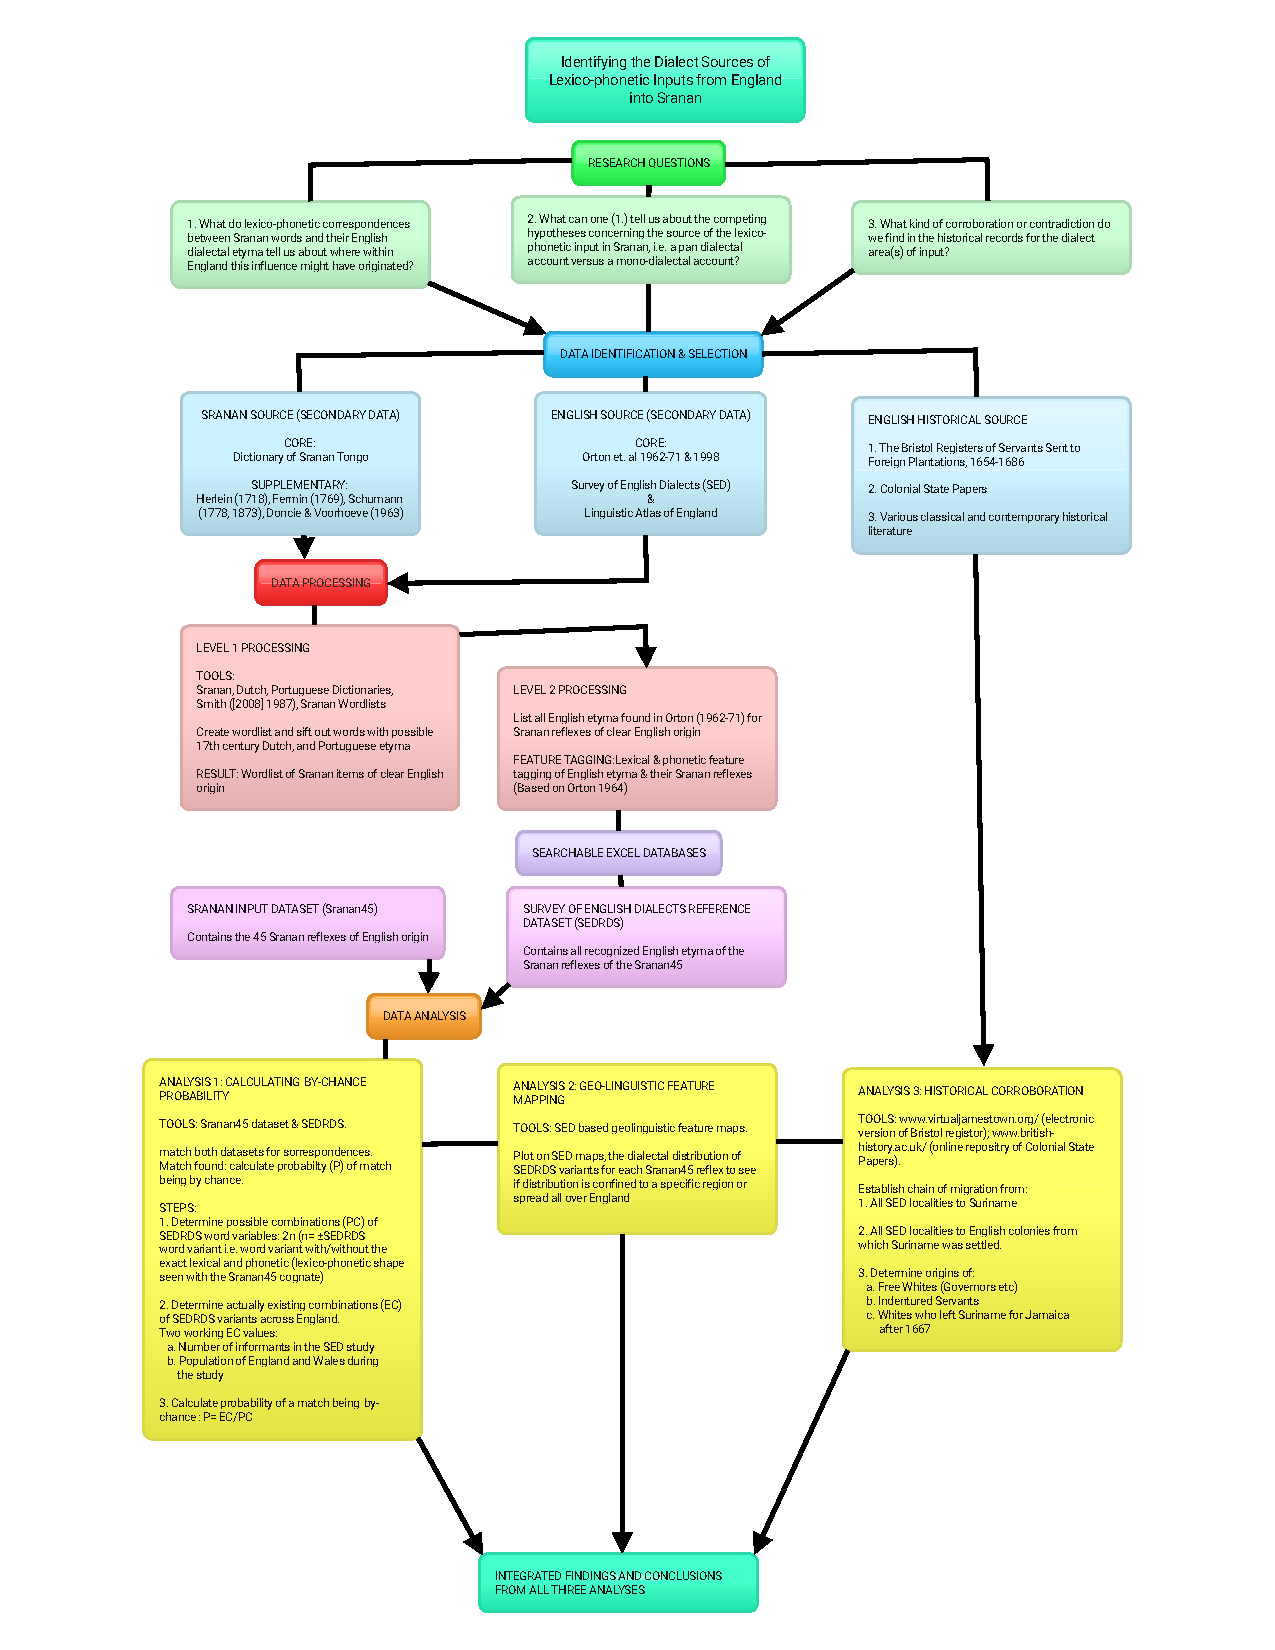
\includegraphics[height=.85\textheight]{figures/researchprocess.pdf}
  %\caption{Some good caption.}
  \caption{\label{Figure 3.1}Research process chart}
\end{figure}
%section 3.4 ends %%%%%%%%%%%%%%%%%%%%%%%%%%%%%%%%%%%%%%%%%%%%%%%%%%%%%%%%%%%%%%%%%%%%
